\chapter{Mise à jour du Plugin}



\noindent
Ce chapitre traite de la correction des bugs existants dans le plugin, de la mise à jour du SDK ainsi que le remplacement des méthodes dépréciées par des méthodes plus récentes.
Enfin, un pipeline a été mis en place sur GitLab afin de tester le plugin à chaque commit.


\section{Correction des bugs}
\noindent Les bugs existants identifiés dans le plugin sont les suivants :

\begin{itemize}
    \item \textbf{Bug 1 :} Le plugin ne permet pas de lancer le script prolog dans la console d'IntelliJ Idea sous Windows.
    \item \textbf{Bug 2 :} Le plugin ne reconnaît pas un opérateur lors de la programmation logique par contrainte.
\end{itemize}

\subsection{Bug 1 : Run dans la console d'IntelliJ Idea sous Windows}
\noindent
Le plugin ne permet pas de lancer le script prolog dans la console d'IntelliJ Idea sous Windows.
\\
\\
\textbf{Description du bug}: Une fois le script prolog compilé et lancé, l'interpréteur prolog boucle sur l'entrée de la console d'IntelliJ Idea ce qui empêche l'utilisateur de saisir des commandes.
\\
\begin{figure}
    \centering
    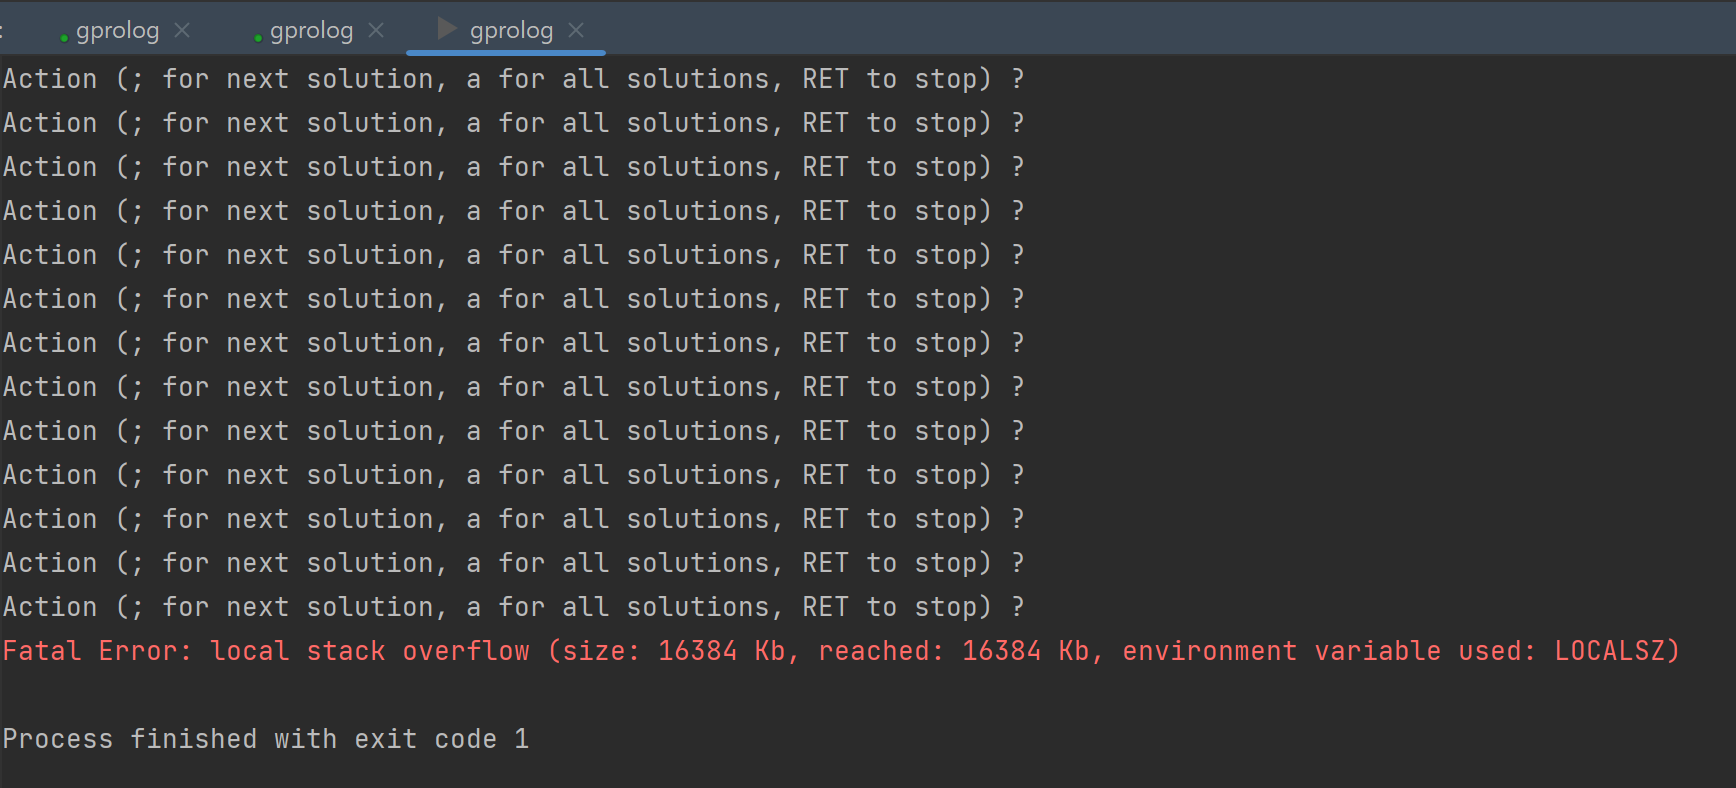
\includegraphics[scale=.85]{images/Bug_1_Windows.png}
    \caption{Image du bug en action dans la console d'IntelliJ Idea}
    \label{fig:bug_1_windows}
\end{figure}

\noindent \textbf{Cause du bug}: La cause n'a pas été clairement identifiée. Cependant, il semble que le problème vienne du fait que le programme prolog s'attend à recevoir des entrées de la console d'IntelliJ Idea et que celle-ci lui envoie des retours à la ligne sans que l'utilisateur ne les ait saisis. Malgré plusieurs tests, je n'ai pas réussi à trouver la cause exacte du problème.
\\
Comme le problème ne se pose pas sous Linux et macOS, il est possible que le problème vienne de la façon dont IntelliJ Idea gère les retours à la ligne sous Windows.
\\
Un test qu'il faudrait faire, serait de faire notre propre programme qui attend des entrées de la console et de voir si le problème se pose également. Si c'est le cas, alors le problème ne vient pas du plugin mais d'IntelliJ Idea. Si le problème ne se pose pas, alors il faudrait chercher la cause du problème dans le plugin ou dans l'intérpréteur prolog.
\\
\\
\textbf{Solution du bug}: Durant l'implémentation de la fonctionnalité permettant d'afficher les erreurs de compilation dans le code, j'ai trouvé une solution fonctionnelle.
\newdoubleline En lançant un invite de commande invisible, il est possible de lancer des commandes via les InputStream et OutputStream de Java. Voici le code permettant de lancer le script prolog :
\begin{lstlisting}[caption={Code permettant de lancer le script prolog}, label={lst:run_script_prolog}]
private Process createWindowsProcess(Path interpreterPath) throws IOException {
    Process p;
    BufferedWriter writer;
    command = "cmd.exe /min";

    if (isInExternalWindow) {
        p = Runtime.getRuntime().exec("cmd.exe /min");
        writer = new BufferedWriter(new OutputStreamWriter(p.getOutputStream()));
        writer.write("cd " + Path.of(getWorkingDir())); //Go to the working directory
        writer.newLine();
        writer.write("set LINEDIT=gui=yes"); //Prevent windows from opening a console
        writer.newLine();
        String query = " --query-goal \"consult('" + Path.of(filePath).getFileName() + "')\"";
        writer.write("start " + interpreterPath.toString() + query); //Launch the compiler
        writer.newLine();
    } else {
        p = Runtime.getRuntime().exec("cmd.exe /min");
        writer = new BufferedWriter(new OutputStreamWriter(p.getOutputStream()));
        writer.write("set LINEDIT=gui=no"); //Prevent windows from opening a console
        writer.newLine();
        writer.write("cd " + Path.of(getWorkingDir())); //Go to the working directory
        writer.newLine();
        writer.write(interpreterPath.toString()); //Launch the compiler
        writer.newLine();
        writer.write("consult('" + Path.of(filePath).getFileName() + "').");
        writer.newLine();
    }

    writer.flush();

    return p;
}
\end{lstlisting}

\subsection{Bug 2 : Opérateur non reconnu lors de la PLC}
\noindent Le plugin ne reconnaît pas un opérateur lors de la programmation logique par contrainte.
\\
\\
\textbf{Description du bug}: L'opérateur "\#=<" n'est pas reconnu en temps que réel opérateur.
\\
\begin{figure}
    \centering
    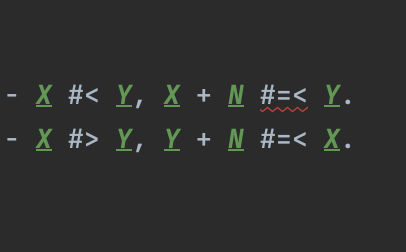
\includegraphics[scale=.85]{images/PLC_error.png}
    \caption{Image du bug en action dans l'éditeur}
    \label{fig:bug_2_plc_op}
\end{figure}

\noindent \textbf{Cause du bug}: Dans le fichier de grammaire BNF, l'opérateur "\#=<" n'est pas présent mais à la place il y a l'opérateur "\#<=" qui, lui, n'existe pas en Prolog.
Il s'agit certainement d'une faute de frappe lors de la rédaction de celle-ci.
\\
\textbf{Solution du bug}: L'opérateur a été ajouté dans la grammaire.

\section{Mise à jour du SDK}
\noindent
Le SDK utilisé pour le développement du plugin est la version 173.0 (2017.3.xxx) de IntelliJ Idea.
Actuellement, la version la plus récente est la 222.4345.14 (2022.2.3) et de nombreuse méthodes utilisées dans le plugin sont dépréciées.

Le but est de mettre à jour le SDK vers une version plus récente afin de pouvoir utiliser les méthodes les plus récentes.

\subsection{Passage du projet en Gradle}
\noindent
Le projet existant n'avait aucun gestionnaire de dépendances et les dépendances étaient gérées manuellement.
Pour lancer le plugin, il fallait donc installer un IDE (par exemple IntelliJ Idea Community) et ajouter les dépendances dans les paramètres du projet.
\\ \noindent Afin de se conformer à la documentation de JetBrains ainsi que de faciliter grandement le développement du plugin, le projet a été migré vers Gradle.
\\\noindent Pour cela, il a fallu ajouter un fichier build.gradle.kts à la racine du projet et configurer les dépendances.
\\ \noindent Afin de pouvoir générer le parser et le lexer, il a fallu ajouter des goals Gradle pour lancer les commandes suivantes :
\begin{lstlisting}
gradle generateParser
gradle generateLexer
\end{lstlisting}


\noindent Ces commandes sont définies dans le fichier build.gradle.kts et permettent de générer le parser et le lexer à partir des fichiers .flex et .bnf.
\begin{lstlisting}
generateLexer {
    source.set("src/main/java/ch/heiafr/intelliprolog/Prolog.flex")
    targetDir.set("src/gen/java/ch/heiafr/intelliprolog/")
    targetClass.set("PrologLexer")
    skeleton.set(file("src/main/java/ch/heiafr/intelliprolog/Prolog.skeleton"))
    purgeOldFiles.set(true)
}


generateParser {

    try {
        val compiledFilesSources =
            files("build/classes/java/main/")
        classpath.from(compiledFilesSources)
    } catch (e: Exception) {
        // Ignore => no compiled files when running the task for the first time
    }

    source.set("src/main/java/ch/heiafr/intelliprolog/Prolog.bnf")
    targetRoot.set("src/gen/java/")
    pathToParser.set("PrologParser.java")
    pathToPsiRoot.set("psi")
    purgeOldFiles.set(false)
}
\end{lstlisting}
\noindent Il a aussi fallu configurer le grammarKit afin de spécifier la version de JFlex.

\begin{lstlisting}
grammarKit {
    jflexRelease.set("1.7.0-2")
}
\end{lstlisting}

Un fichier settings.properties a également été ajouté afin de spécifier :
\begin{itemize}
    \item Le nom du plugin
    \item Le groupe du plugin
    \item La version du plugin
    \item La version minimum d'IntelliJ Idea requise pour lancer le plugin
    \item La plateforme cible (Ultimate, Education, Community) pour lancer le plugin
    \item La version de la plateforme cible pour lancer le plugin
    \item La dépendance de la plateforme cible
    \item La version de Java utilisée
    \item La version cible de Java pour le Kotlin
    \item La version de Gradle utilisée
\end{itemize}

Le fichier settings.properties est lu par le fichier build.gradle.kts afin de configurer le plugin lors de la compilation ainsi que lors de la création du ZIP du plugin.

\subsection{Le problème du GrammarKit}
\noindent
Le plugin utilise le GrammarKit afin de générer le parser et le lexer à partir des fichiers .flex et .bnf.
\\ \noindent Le problème est que pour pouvoir générer le parser et le lexer, il faut que le plugin soit compilé et pour que le plugin soit compilé, il faut que le parser et le lexer soient générés\ldots
\newdoubleline
Pour résoudre ce problème, j'ai cherché une solution sur de nombreux forums et malgré plusieurs tentatives, je n'ai pas réussi à trouver de solution fonctionnelle aussi bien en local que sur la CI.
\\ \noindent J'ai donc décidé d'écrire mes propres "goals" Gradle afin de générer le parser et le lexer en 3 étapes :
\begin{enumerate}
    \item Génération du parser et du lexer
    \item Compilation du plugin
    \item Génération du parser et du lexer
\end{enumerate}


\begin{lstlisting}
register("compileAndRegenerate") {
    dependsOn("compileJava")
    finalizedBy("generateParser")
}

register("initProject") {

    doFirst {
        generateParser.get().generateParser()
        generateLexer.get().generateLexer()
        println("Classes generated")
    }
    finalizedBy("compileAndRegenerate")
}
\end{lstlisting}

\noindent \textbf{Attention :} lorsque le projet est cloné, il faut lancer la commande suivante afin de générer le parser et le lexer :
\begin{lstlisting}
    gradle initProject
\end{lstlisting}

\noindent J'ai du implémenter certaines méthodes dans un fichier "PrologNamedElementHelperImpl.java" afin de pouvoir générer le parser et le lexer sans erreur de compilation.

\begin{lstlisting}
public class PrologNamedElementHelperImpl extends ASTWrapperPsiElement implements PrologNamedElement {

  public PrologNamedElementHelperImpl(@NotNull ASTNode node) {
    super(node);
  }

  @Override
  public @Nullable PsiElement getNameIdentifier() {
    return null;
  }

  @Override
  public PsiElement setName(@NlsSafe @NotNull String name) throws IncorrectOperationException {
    return null;
  }
}
\end{lstlisting}


\section{Mise en place de la CI}
\noindent La CI a été mise en place sur GitLab afin de tester le plugin à chaque commit.
Celle-ci permet aussi de créer une release entièrement automatisée lors de la création d'un tag sur le dépôt GitLab.
\\ \noindent La pipeline est définie dans le fichier .gitlab-ci.yml à la racine du projet.
\newdoubleline
\noindent Le pipeline est composé de 3 jobs :
\begin{itemize}
    \item \textbf{Build} : Génération du parser et du lexer, compilation du plugin
    \item \textbf{Test} : Lancement des tests unitaires
    \item \textbf{Release} : Création d'une release du plugin (uniquement sur les tags)
\end{itemize}

\begin{figure}[H]
    \centering
    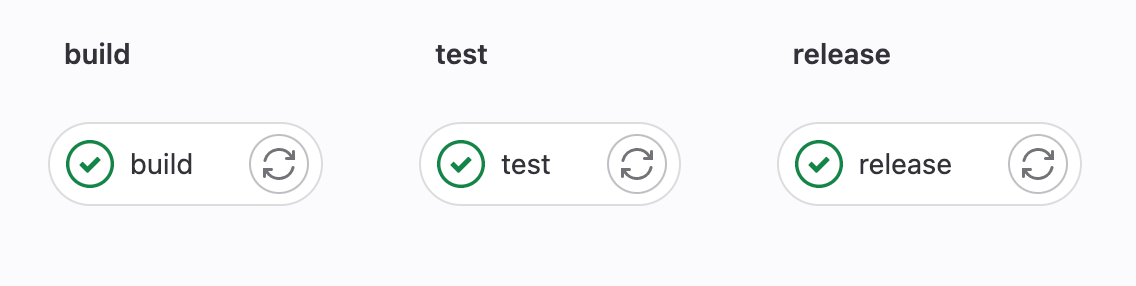
\includegraphics[width=0.8\textwidth]{images/Pipeline.png}
    \caption{Pipeline de la CI}
    \label{fig:gitlab-ci}
\end{figure}
